\documentclass{article}
\usepackage[utf8]{inputenc}
\usepackage{graphicx}
\usepackage{titling}
\usepackage{titlesec}
\usepackage{booktabs}
\usepackage{fancyhdr}
\usepackage{lipsum}
\usepackage{comment}
\usepackage{enumitem}
\usepackage{listings}
\usepackage{xcolor}
\usepackage{longtable}
\usepackage{cite}
\usepackage{pgfgantt}
\usepackage{amsmath}
\usepackage{tikz}
\usepackage[margin=1in]{geometry}
\usetikzlibrary{calc}


\lstdefinestyle{pidstyle}{
    basicstyle=\ttfamily\footnotesize,
    breaklines=true,
    escapechar=\#, % Define escape character for inline LaTeX commands
    linewidth=\textwidth,
    basicstyle=\ttfamily\scriptsize
}

\renewcommand{\maketitle}{%
  \begin{leftmark}
    \vspace*{\baselineskip} % Add a bit of vertical space

%    \includegraphics[width=4cm]{example-image-a} % Add an image before the title. you will need to replace the image path with your own

%    \vspace{0.5cm} % Add vertical space before title

    \textbf{\fontsize{18}{36}\selectfont \thetitle} % Font Size and Bold Title

     \vspace{0.05cm} % Add vertical space before subtitle
%    \textit{\Large \theauthor}  % Subtitle / Author
    \vspace{\baselineskip} % Add vertical space after subtitle
     \rule{\textwidth}{0.4pt} % Add a horizontal line

   \end{leftmark}
%    \thispagestyle{empty} % Prevent header/footer on the title page
}


% Section Formatting
\titleformat{\section}
  {\normalfont\fontsize{18}{22}\bfseries} % Font and style
  {\thesection}         % Section number
  {1em}                   % Horizontal space after section number
  {}                     % Code before the section name
  []                     % Code after the section name

\titleformat{\subsection}
  {\normalfont\fontsize{14}{18}\bfseries} % Font and style
  {\thesubsection}         % Subsection number
  {1em}                   % Horizontal space after subsection number
  {}                     % Code before the subsection name
  []                     % Code after the subsection name

\setlength{\parindent}{0pt}

\title{Computing platforms (Spring 2025)\newline
week 2}
\author{Juha-Pekka Heikkilä}



\pagestyle{fancy}
\fancyhf{}

\renewcommand{\headrulewidth}{0pt}

\newcommand{\footerline}{\makebox[\textwidth]{\hrulefill}}

\newcommand{\footercontent}{%
    \begin{tabular}{@{}l@{}}
        \footerline \\
        \leftmark \hfill \rlap{\thepage}
    \end{tabular}
}

\fancyfoot[C]{\footercontent}


\newcommand{\exercise}[1]{
    \section*{Exercise #1}
    \markboth{Exercise #1}{}
}



\begin{document}
\maketitle


\exercise{1}
{\bf Multicore. Suppose a single application is running on
a multicore system with 16 processors. If 20\% of the code
is inherently serial, what is the performance gain over
a single processor system? What would it be if only 2\% of
the code would be inherently serial?}
\newline

Using Amdahl's Law \cite{stallings4.3}:
\[
S = \frac{1}{(1 - f) + \frac{f}{N}}
\]
where:
\begin{itemize}
    \item \( 1 - f \): Fraction of the code that is inherently serial.
    \item \( f \): Fraction of the code that is parallelizable.
    \item \( N = 16 \): Number of processors.
\end{itemize}

\begin{enumerate}[label=\textbf{\alph*})]
    \item \textbf{20\% Serial Code (\( 1 - f = 0.2 \), \( f = 0.8 \))}

    Substitute into the formula:
    \[
    S = \frac{1}{(1 - 0.8) + \frac{0.8}{16}} = \frac{1}{0.2 + 0.05} = \frac{1}{0.25} = 4
    \]

    \textbf{Performance Gain:} \( S = 4 \).

    \item \textbf{2\% Serial Code (\( 1 - f = 0.02 \), \( f = 0.98 \))}

    Substitute into the formula:
    \[
    S = \frac{1}{(1 - 0.98) + \frac{0.98}{16}} = \frac{1}{0.02 + 0.06125} = \frac{1}{0.08125} \approx 12.31
    \]

    \textbf{Performance Gain:} \( S \approx 12.31 \).
\end{enumerate}

\newpage

\exercise{2}


We have four jobs that arrive at time 0
\[
\noindent
\begin{aligned}    
A &= 5\text{ ms} \quad \\
B &= 6\text{ ms} \quad \\
C &= 4\text{ ms} \quad \\
D &= 1\text{ ms}
\end{aligned}
\]
All are CPU-bound and we ignore context switch overhead.

\subsection*{(a) Round-Robin with 2 ms time slice}

%\noindent
%\textbf{Timeline Chart:}

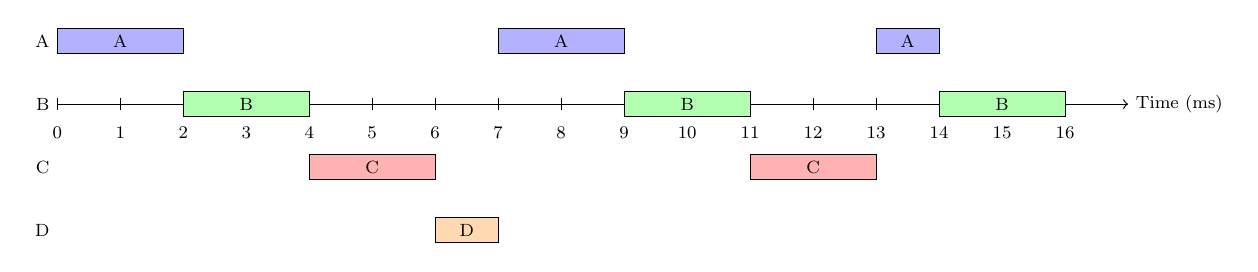
\begin{tikzpicture}[scale=0.8, transform shape, font=\footnotesize]
  % Horizontal axis
  \draw[->] (0,0) -- (17,0) node[right]{Time (ms)};
  % Ticks from 0..16
  \foreach \x in {0,1,2,...,16} {
    \draw (\x,0.1) -- (\x,-0.1) node[below=4pt]{\x};
  }

  \def\drawTime#1#2#3#4#5{
    \draw[fill=#4,draw=black] 
      (#1,#3+0.2) rectangle (#2,#3-0.2) 
      node[midway]{#5};
  }

  % Round-Robin intervals (see bullet list above):

  % (y=1.0)
  \drawTime{0}{2}{1.0}{blue!30}{A}
  \drawTime{7}{9}{1.0}{blue!30}{A}
  \drawTime{13}{14}{1.0}{blue!30}{A}

  % B (y=0.0)
  \drawTime{2}{4}{0.0}{green!30}{B}
  \drawTime{9}{11}{0.0}{green!30}{B}
  \drawTime{14}{16}{0.0}{green!30}{B}

  % C (y=-1.0)
  \drawTime{4}{6}{-1.0}{red!30}{C}
  \drawTime{11}{13}{-1.0}{red!30}{C}

  % D (y=-2.0)
  \drawTime{6}{7}{-2.0}{orange!30}{D}

  % Labels for each job on the left
  \node[left] at (0,1.0) {A};
  \node[left] at (0,0.0) {B};
  \node[left] at (0,-1.0) {C};
  \node[left] at (0,-2.0) {D};
\end{tikzpicture}

\vspace{1em}
\noindent
\textbf{Turnaround times:}
\[
\begin{aligned}
A &\to 14\quad \\
B &\to 16\quad \\
C &\to 13\quad \\
D &\to 7
\end{aligned}
\]

\noindent
\textbf{Average TAT} = \(\frac{14 + 16 + 13 + 7}{4} = 12.5\,\text{ms}\)

\vspace{1em}


\subsection*{(b) First-come-first-served}

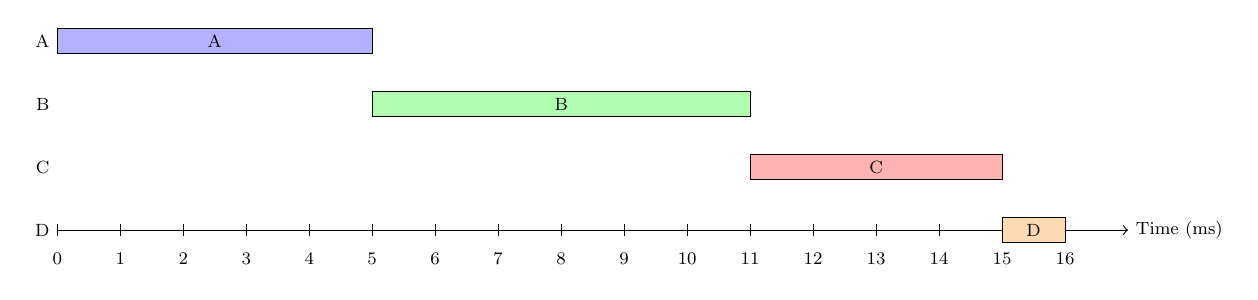
\begin{tikzpicture}[scale=0.8, transform shape, font=\footnotesize]
  \draw[->] (0,0) -- (17,0) node[right]{Time (ms)};
  \foreach \x in {0,1,2,...,16} {
    \draw (\x,0.1) -- (\x,-0.1) node[below=4pt]{\x};
  }

  \def\drawTime#1#2#3#4#5{
    \draw[fill=#4,draw=black] 
      (#1,#3+0.2) rectangle (#2,#3-0.2) 
      node[midway]{#5};
  }

  \drawTime{0}{5}{3.0}{blue!30}{A}
  \drawTime{5}{11}{2.0}{green!30}{B}
  \drawTime{11}{15}{1.0}{red!30}{C}
  \drawTime{15}{16}{0.0}{orange!30}{D}

  \node[left] at (0,3.0) {A};
  \node[left] at (0,2.0) {B};
  \node[left] at (0,1.0) {C};
  \node[left] at (0,0.0) {D};
\end{tikzpicture}

\vspace{1em}
\noindent
\textbf{Turnaround times:}    
\[
    \begin{aligned}
        A &\to 5 \\
        B &\to 11 \\
        C &\to 15 \\
        D &\to 16 \\
    \end{aligned}
\]

\noindent
\textbf{Average TAT} = \(\frac{5 + 11 + 15 + 16}{4} = 11.75\,\text{ms}\)

\newpage

\subsection*{(c) Shortest-job-first}

Order by shortest runtime first: \(D \to C \to A \to B.\) \newline


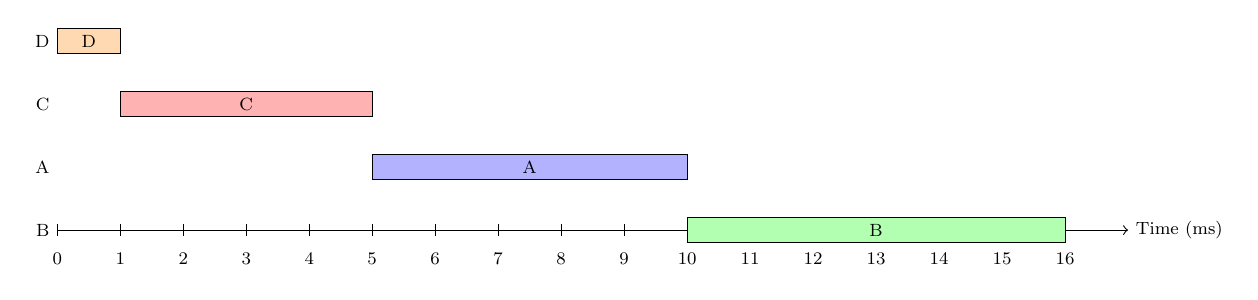
\begin{tikzpicture}[scale=0.8, transform shape, font=\footnotesize]
  \draw[->] (0,0) -- (17,0) node[right]{Time (ms)};
  \foreach \x in {0,1,2,...,16} {
    \draw (\x,0.1) -- (\x,-0.1) node[below=4pt]{\x};
  }

  \def\drawTime#1#2#3#4#5{
    \draw[fill=#4,draw=black] 
      (#1,#3+0.2) rectangle (#2,#3-0.2) 
      node[midway]{#5};
  }

  \drawTime{0}{1}{3.0}{orange!30}{D}
  \drawTime{1}{5}{2.0}{red!30}{C}
  \drawTime{5}{10}{1.0}{blue!30}{A}
  \drawTime{10}{16}{0.0}{green!30}{B}

  \node[left] at (0,3.0) {D};
  \node[left] at (0,2.0) {C};
  \node[left] at (0,1.0) {A};
  \node[left] at (0,0.0) {B};
\end{tikzpicture}

\vspace{1em}
\noindent
\textbf{Turnaround times:}
\[
\begin{aligned}
    D &\to 1 \\
    C &\to 5 \\
    A &\to 10 \\
    B &\to 16 \\
\end{aligned}
\]

\textbf{Average TAT} = \(\frac{1 + 5 + 10 + 16}{4} = 8\,\text{ms}\)



\newpage
\bibliographystyle{plain}
\bibliography{references}
\end{document}